\documentclass[11pt]{article}

\usepackage{mathpazo}
\usepackage{upgreek}
\usepackage{fullpage}
\usepackage{graphicx}
\usepackage{booktabs}                      % beautiful tables
\usepackage{caption}                       % allow multi-line captions
\usepackage{afterpage}
\usepackage{tabularx}
\usepackage{enumitem}
\usepackage{longtable}
\usepackage{parskip}

\setlength{\parskip}{\baselineskip}
\setlength{\parindent}{0pt}

%% and here the glossaries package is... ------------------
% \usepackage{glossaries}
% \makeglossaries

% % regular acronym
% \newcommand{\acr}[1]{\gls{#1}}

% % plural acronym
% \newcommand{\acrpl}[1]{\glspl{#1}}

% % short version acronym (for captions, titles, etc)
% \newcommand{\acrsh}[1]{\glsentryshort{#1}}

% % short and plural acronym (for captions, titles, etc)
% \newcommand{\acrshpl}[1]{\glsentryshortpl{#1}}

% % creates acronym and also helper commands to ease use during writing
% \newcommand\makeacronym[4][]{
%   \newacronym[#1]{#2}{#3}{#4}
%   \expandafter\newcommand\csname #2\endcsname[1][]{%
%     \csname acr##1\endcsname{#2}\xspace%
%   }
% }

%% to make a ref for table and figures. Notice label prefix, which
%% means you should include those in the labels when including the
%% figure, but you don't need to put them when using the commands
%% below. This guaranties that you are not misplacing a figure in the
%% place of a table, or the other way around.
\newcommand{\figref}[1]{Figure~\ref{fig:#1}}
\newcommand{\tabref}[1]{Table~\ref{tab:#1}}
\newcommand{\secref}[1]{Section~\ref{sec:#1}}

% links and glossaries

\usepackage{hyperref} % hyperlinks, always last but glossaries


\title{ETL Readout Board Design}
\author{Indara Suarez, Daniel Spitzbart, Andrew Peck, Eric Hazen, Shouxiang Wu
  \\
  \\ \Large{\textbf{Boston University}}}

\date{\today}

\begin{document}

\maketitle

\tableofcontents

\section{Introduction to the Flipped Module Design}

This document describes an alternative of the ETL module and service hybrid design to the TDR design. In this proposal the silicon sensor is located below the read out chip (ETROC), essentially flipping the TDR module on its head. A PCB can be mounted (glued) on top of the ETROC.

Describe the flipped module design

How many flavors of SH (I think this is consistent with the TDR right?)

Picture of the design similar to the one on the TDR

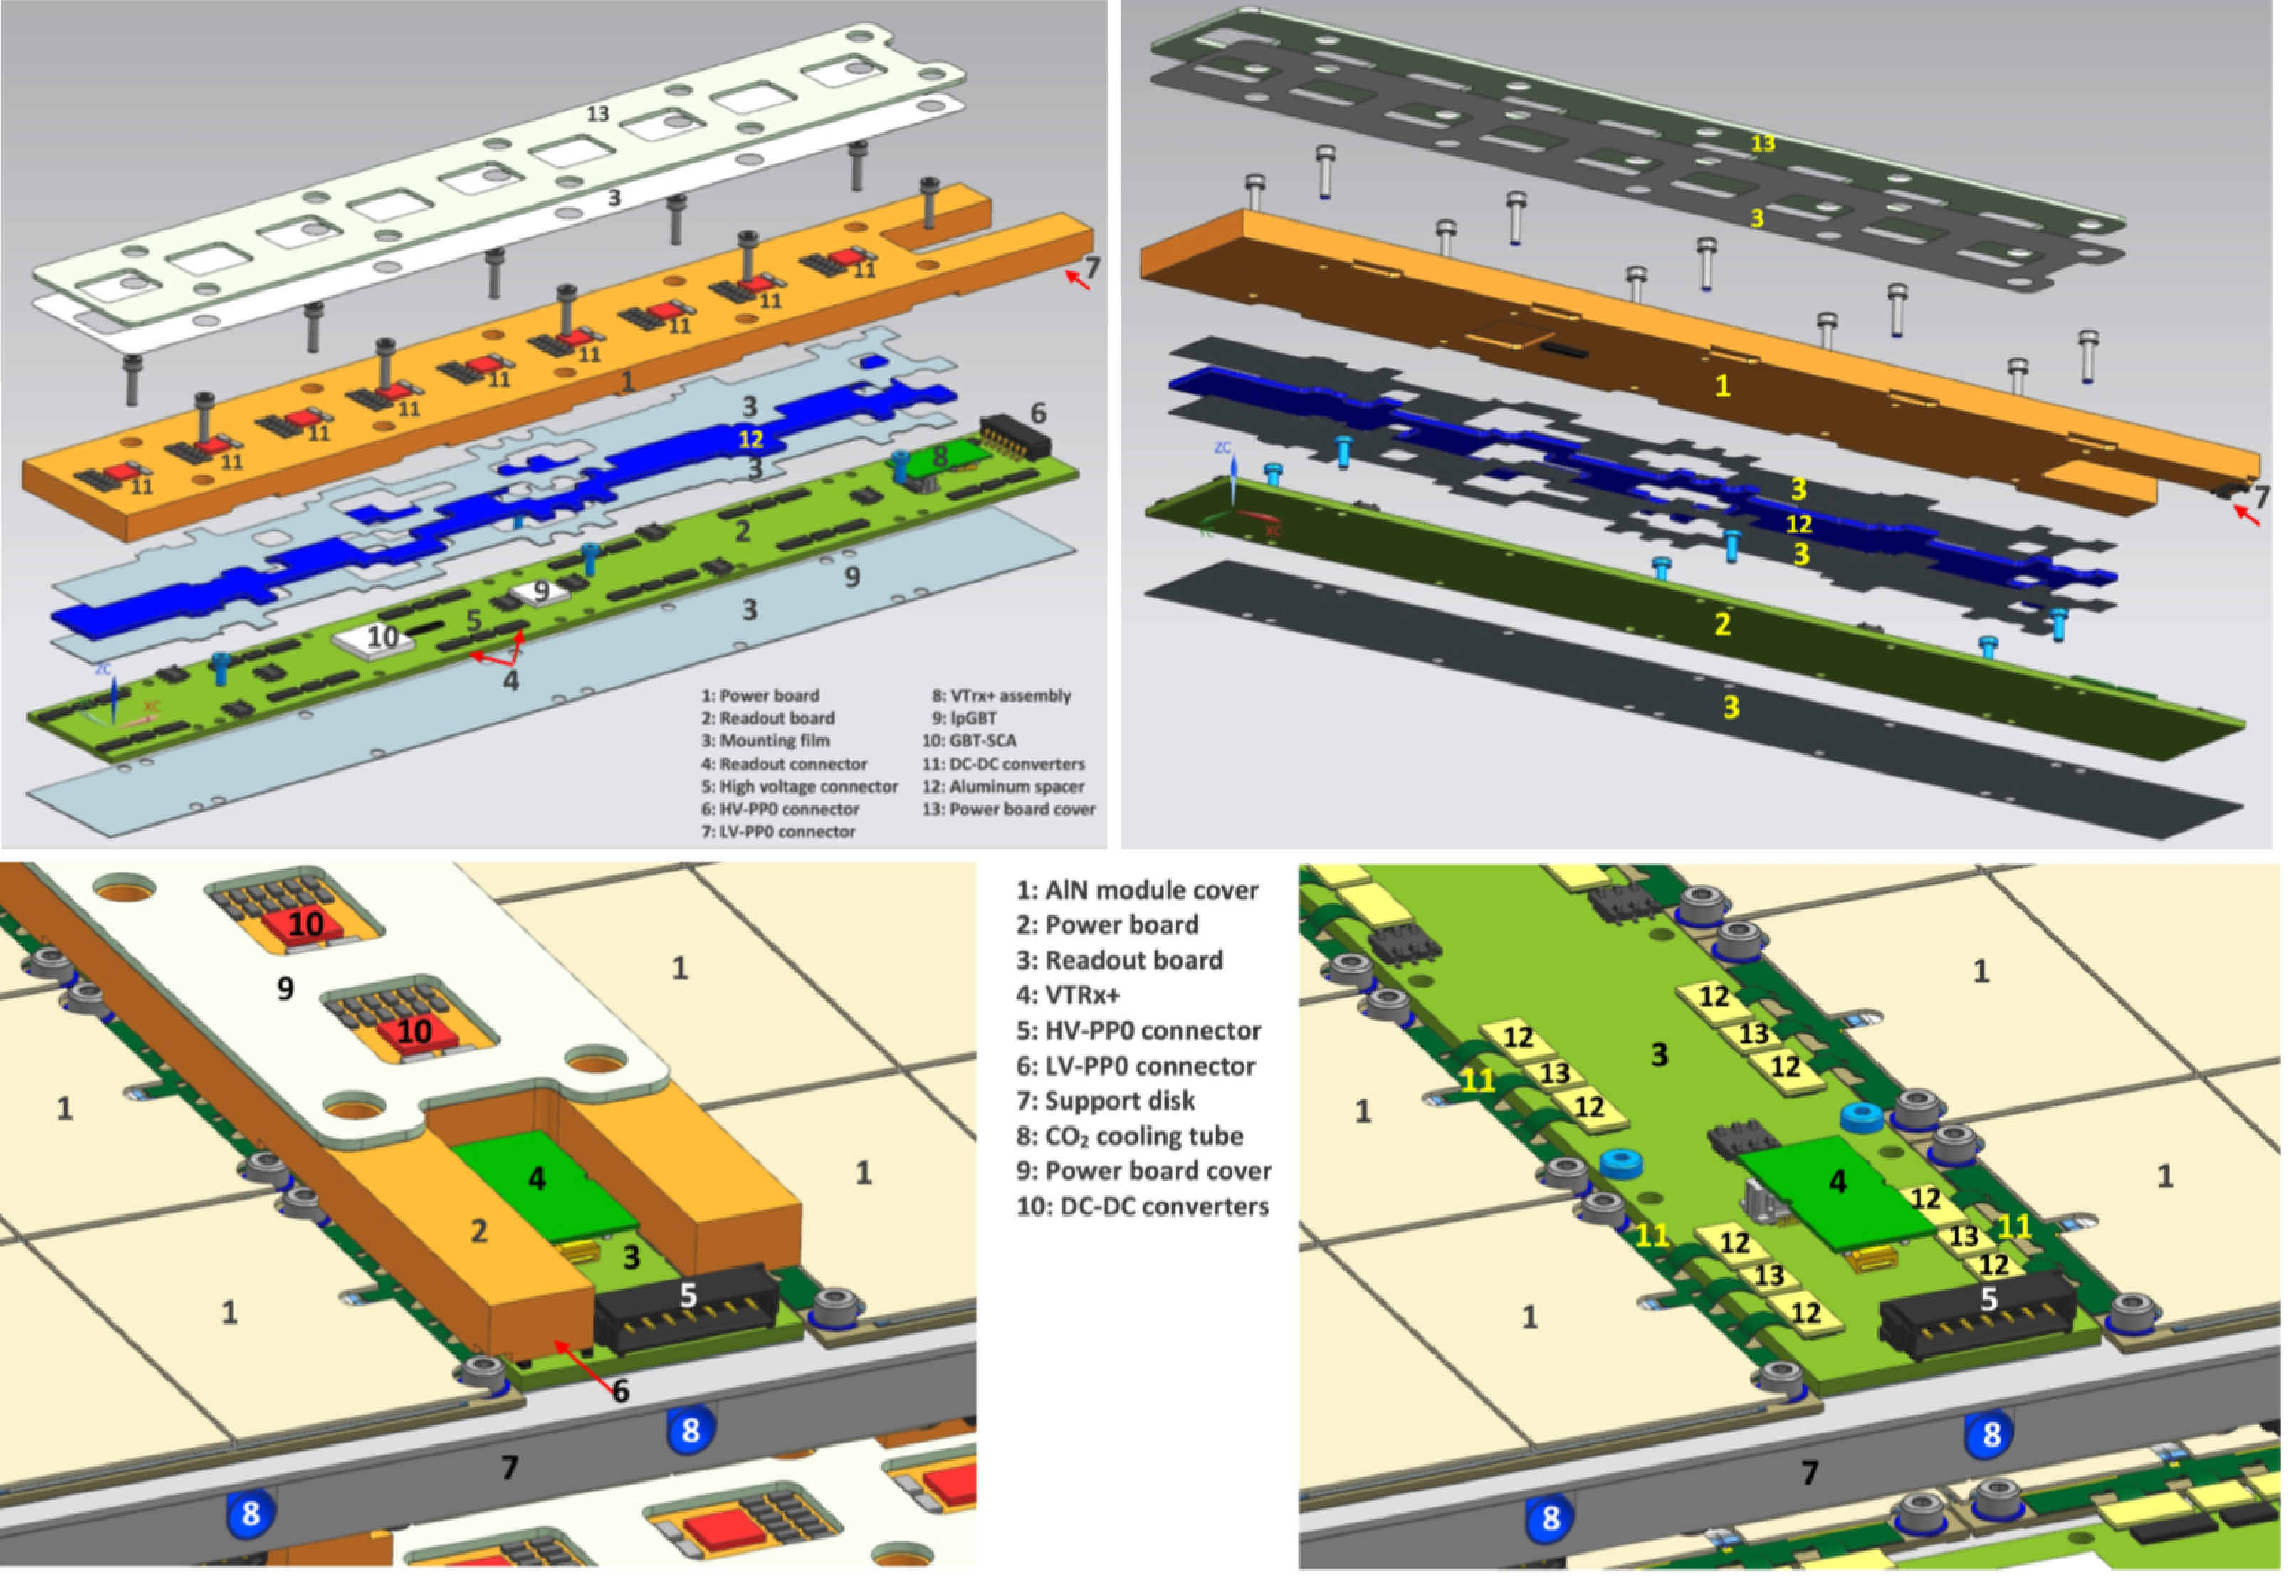
\includegraphics[width=\linewidth]{figures/image7.pdf}

\emph{Figure 1: Top: Exploded views of the service hybrid showing its various components. Bottom: Service hybrid mounted between two modules, with the power board visible on top (left), and the service hybrid showing the readout board and components (right).}

The expected radiation environment for various regions are shown in Table 1, and they roughly correspond to being populated by the 6-module boards in the area at $>$1$\times$10$^{15}$ n/cm$^{2}$, and the rest is organized such that to optimize the area coverage of the detector with sensors. The layout of modules and service hybrids on the surface of the ETL wedges is presented in Figure 2.

\begin{table}
  \centering
  \caption{Table 1: Nominal radiation doses and fluences at various locations of the timing layers after 3000 fb$^{-1}$. The last two columns show the radiation levels providing a safety margin of a factor 1.5. The fluence is normalized to 1 MeV neutron equivalent in silicon.}
  \label{table:radiationField}
  \begin{tabular}{ c c c c c c }
    Region & $\eta$ & R (cm) & z (cm) & Fluence (cm$^{-2}$) & Dose (kGy) \\
    \midrule
    barrel & 0.0    & 117    & 0      & 1.7$\times 10^{14}$ & 16         \\
    barrel & 1.15   & 117    & 170    & 1.9$\times 10^{14}$ & 21         \\
    barrel & 1.45   & 117    & 240    & 2.0$\times 10^{14}$ & 25         \\
    endcap & 1.6    & 127    & 304    & 1.1$\times 10^{14}$ & 25         \\
    endcap & 2.0    & 84     & 304    & 2.4$\times 10^{14}$ & 75         \\
    endcap & 2.5    & 50     & 304    & 6.6$\times 10^{14}$ & 260        \\
    endcap & 3.0    & 30     & 304    & 1.7$\times 10^{15}$ & 690        \\
  \end{tabular}
\end{table}

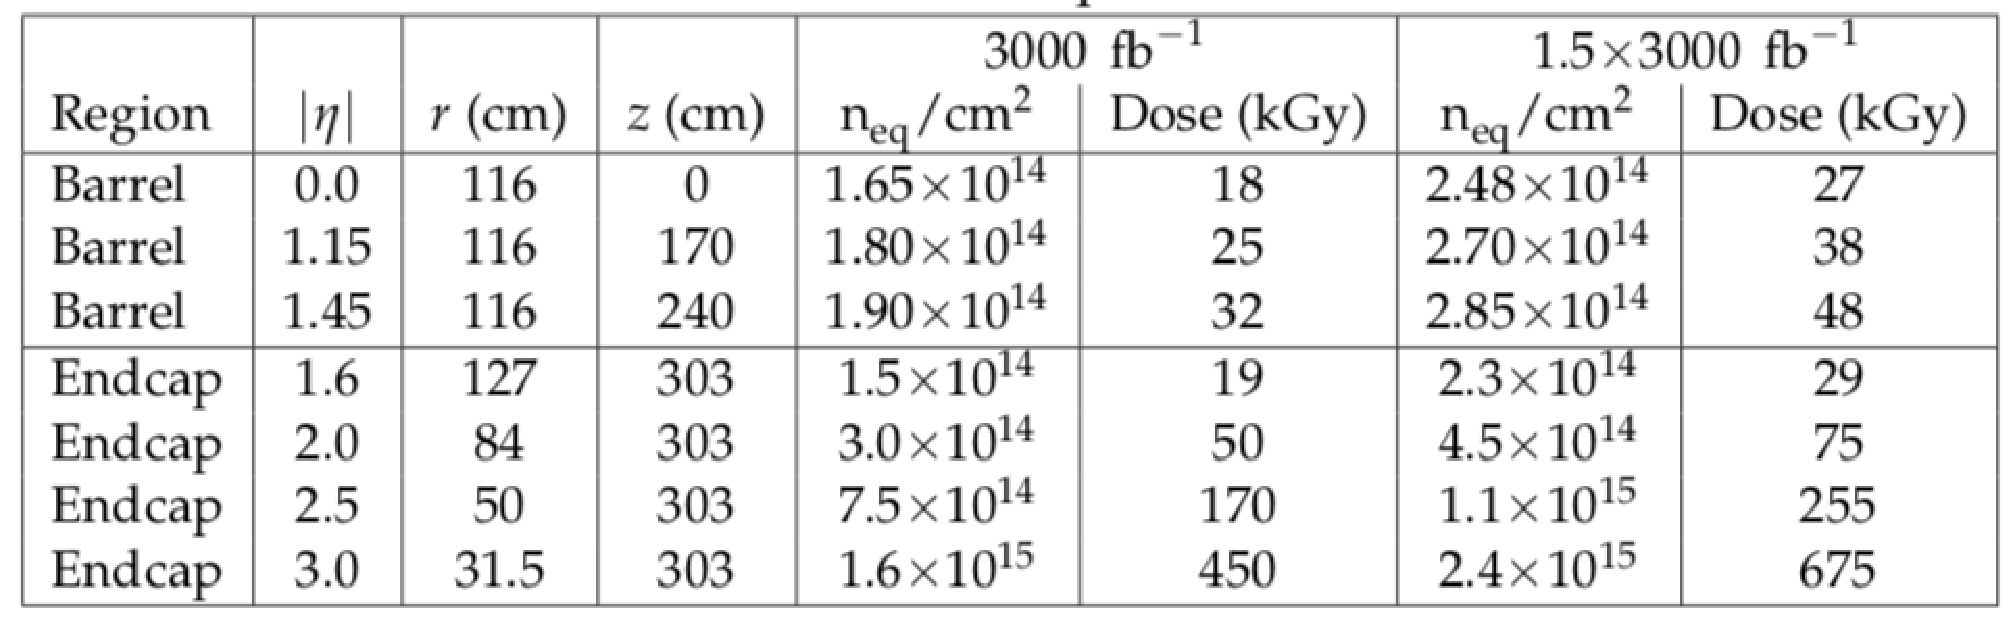
\includegraphics[width=\linewidth]{figures/image4.pdf}

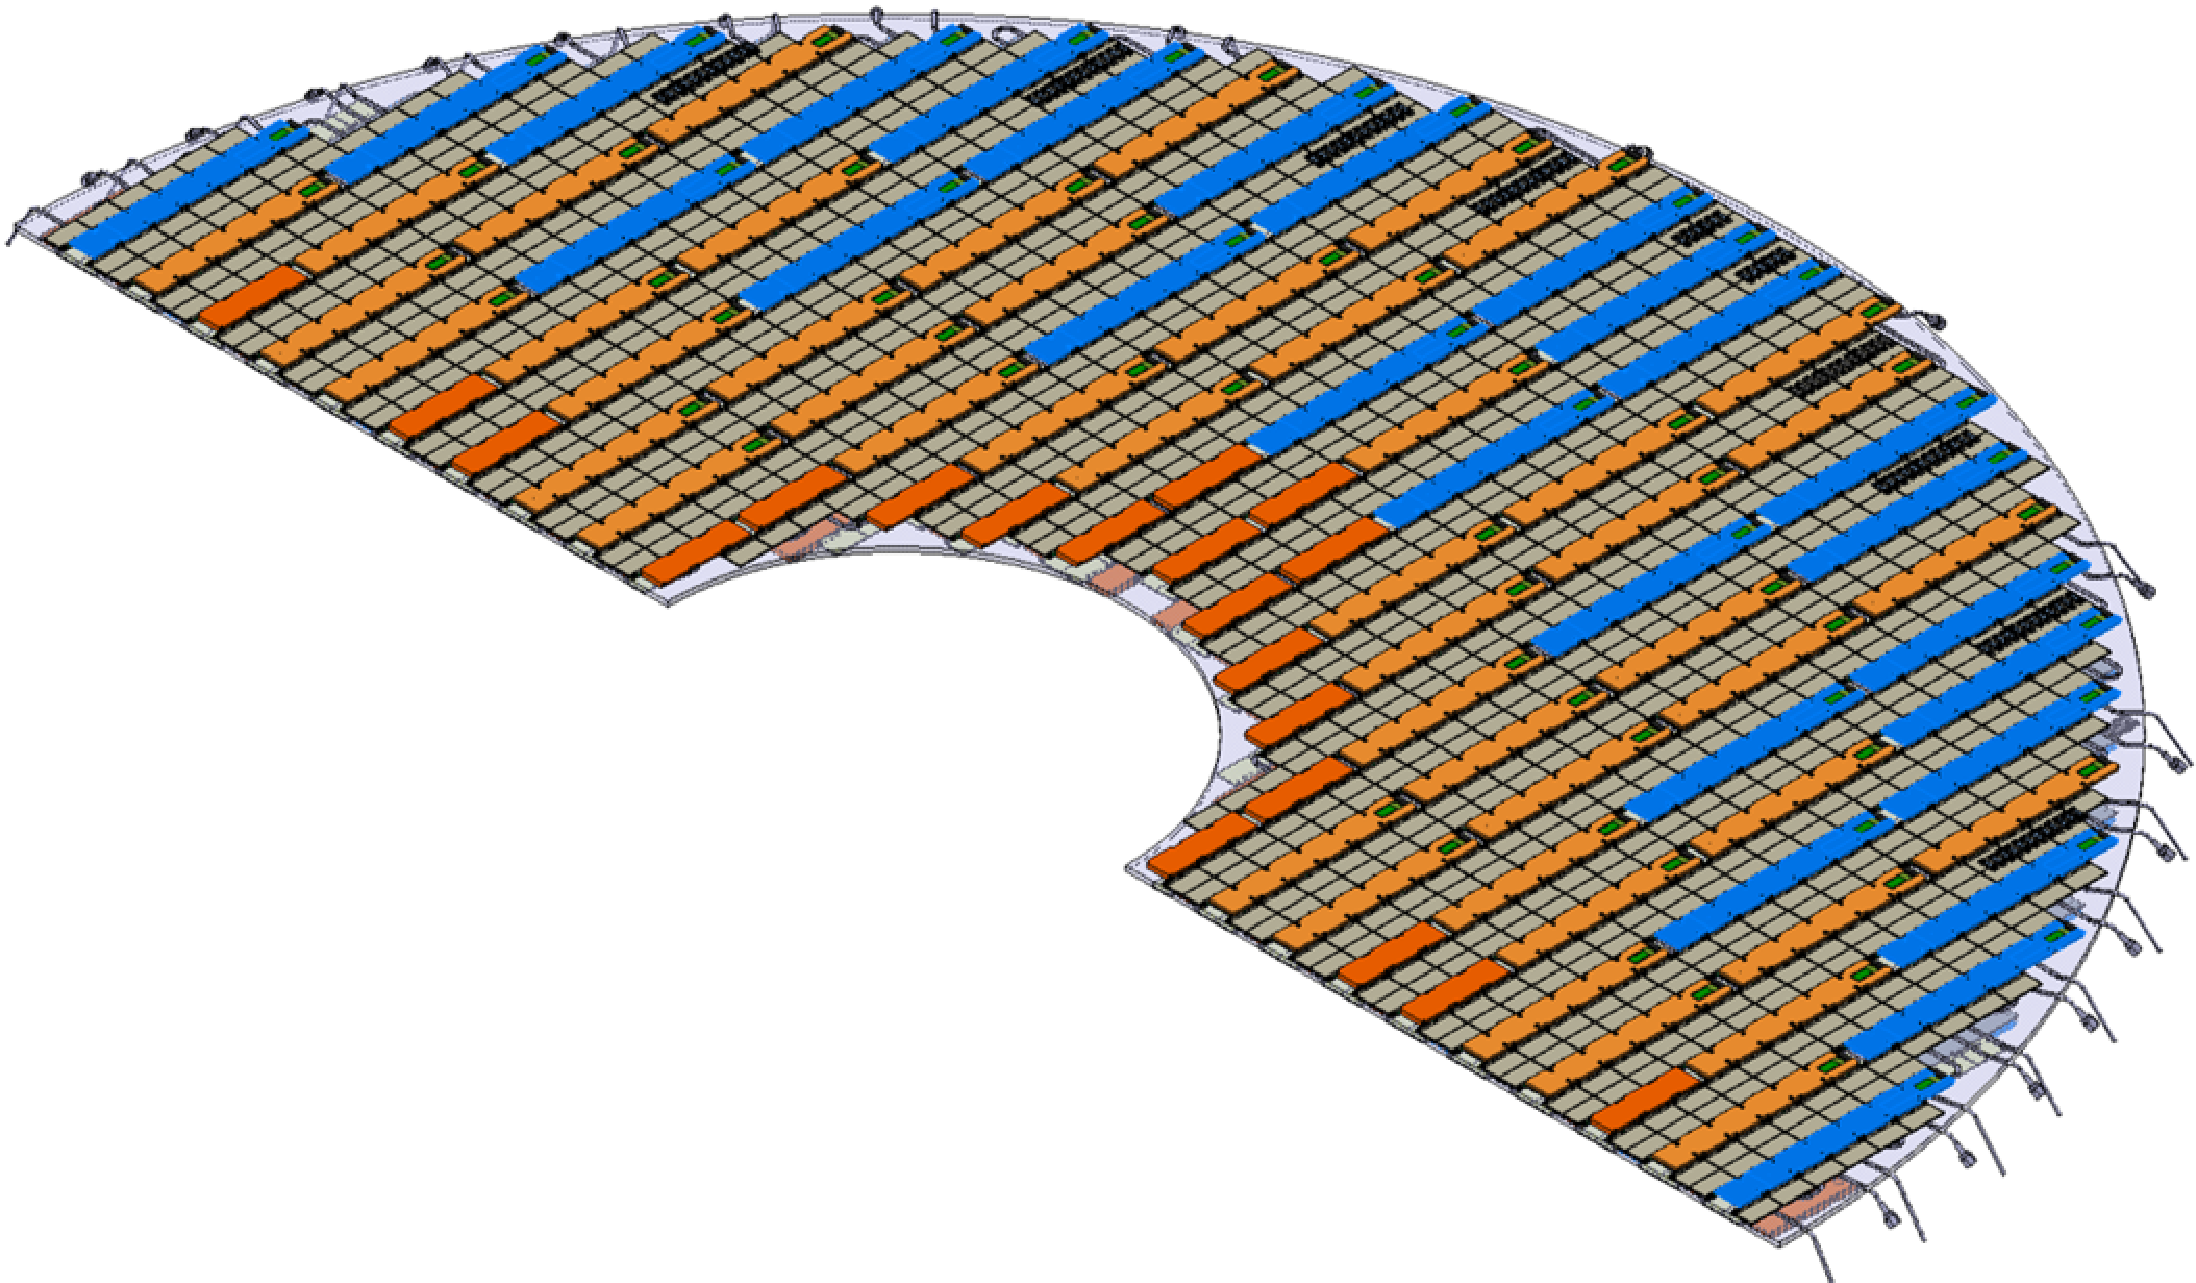
\includegraphics[width=\linewidth]{figures/image3.pdf}

\emph{Figure 2: Layout of various kinds of SH on an ETL half-disk}

Can you update this table?

\begin{table}
  \caption{List of the number of each type of component used in the full ETL detector.}
  \centering
  \begin{tabular}{ l c c }
    Component type             & Number per wedge & Total number \\
    \midrule
    LGADs                     & 1,136            & 18,176       \\
    ETROCs                    & 2,272            & 36,352       \\
    1-sensor modules          & 80               & 1,280        \\
    2-sensor modules          & 528              & 8,448        \\
    Full-size service hybrids & 87               & 1,392        \\
    Half-size service hybrids & 22               & 352          \\
    lpGBTs, VTRX, SCA         & 109              & 1,744        \\
    DC-DC converters          & 893              & 14,288       \\ %9 per full-size and 5 per half-size
  \end{tabular}
  \label{tab:ETLNumberOfComponents}
\end{table}

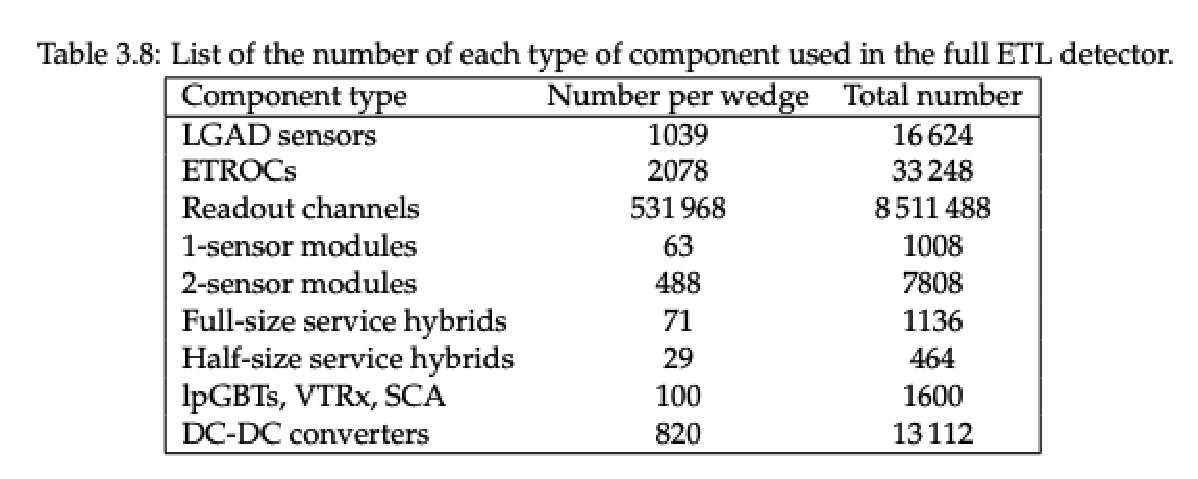
\includegraphics[width=\linewidth]{figures/image1.pdf}

\section{Changes to the Module Design}

(not sure if this is better with the section above)

Here talk about the specific module

Things related to cooling and the PCB

Bring up any Issues with modules that we may have

\section{Service Hybrid Requirements}

I would update only the sections that are different from the previous
document. I think there is a new selection of connectors, that should
get updated.

\section{Specifications for the Power Board}

I guess we assume this doesn't change and just in the section above put how much area is available for the PB?

\section{Specifications for the Readout Board}

I also think most of this is not changing.

(below is what we had in the previous document)

The most important functions for the RB are:

\begin{itemize}
  \item Distribute the lpGBT recovered and phase-locked system clock to the ETROC ASICs with a minimal time jitter degradation.
  \item Provide good signal integrity paths for the 320Mbps ETROC to lpGBT readout data streams. The RB design should allow for data output interface between ETROC to lpGBT to run up at speeds from 160 Mbps to
    320 Mbps.
\end{itemize}

Besides those two critical functions, RB performs several more:

\begin{itemize}
  \item Distributes fast commands from lpGBT to ETROCs using e-link channels, mirrored e-links will be used to achieve a higher throughput of 320 Mbps [14], [15]. A preliminary list of fast commands includes BC0/Orbit Reset, DAQ-Resync, Link-Reset, L1A, CalibrationReq, CalibrationL1A, OrbitCounterReset, and PixelMask, and is presented in Ref. [15].
  \item Provides configuration channels to ETROCs using I2C masters available in SCA
  \item Slow control and monitoring, utilizing more of the SCA resources
  \item LV distribution and filtering (if needed) from the PB and to the on-board VTRX+/lpGBT/SCA and all ETROCs on the attached detector modules.
  \item Current plan is to have several versions with 12, 24 and possibly 28 ETROCs per RB. Those numbers allow for the best use of the lpGBT resources and to have more data bandwidth per ETROC for higher event rate locations at lower R. The optimization studies presented in Ref [3] will need to identify the optimal configuration that minimizes the kinds of SH, while maintaining the detector coverage with sensors and maintaining radiation tolerance.
  \item BV distribution from an input connector and to the attached detector modules. Best achievable filtering scheme should be designed to ensure additional timing jitter for the detector signals does not exceed 5ps rms. The BV connector should be able to supply up to 800 V voltage per module at 20 $\mu$A per sensor. Up to 6 different bias voltage lines are envisioned for the nominal size of the SH, each BV being applied to two modules.
\end{itemize}

These functions performed by the board have to be incorporated in the smallest package that fits into the overall dimension requirements listed above.

The lpGBT will be used to distribute clock, fast commands and collect data from connected ETROC ASICs. The list of available input/outputs per lpGBT is below.

\begin{itemize}
  \item Clock: 29 e-clocks available, plan to use 40MHz. Since up to 28 ETROCs are planned to be connected to a single lpGBT, one e-clock is connected to one ETROC by default.
  \item Fast commands: 16 output e-links available, combined in 4 groups. A single e-link will be connected to two ETROCs. Since all ETROCs should receive the same commands, we will increase the basic output e-link speed from 80 to 320 Mbps by turning on only one e-link in the group (4 e-links @ 320Mbps) and mirroring the rest of them.
  \item Data readout - up to 28 input e-links running at 320Mbps, while for the smaller SH version with 12 connected ETROCs, e-links can operate at 640Mbps
\end{itemize}

The baseline for RB will support up to 320Mbps for the down eLinks to give ETROC designers as much flexibility as possible at the cost of no hardware changes. For the up eLinks direction (from ETROC to backend), the current design (1 LpGBT) will support two scenarios:

\begin{itemize}
  \item Up to 640 Mbps with no trigger present
  \item 320 Mbs with the addition of a 320Mbps trigger eLink
\end{itemize}

This is based on a simulation study of the occupancy of each ASIC (with 200 PU interactions merged with ttbar events). This study showed that all but the highest $\eta$ regions have an average occupancy corresponding to 160 Mbps. At the higher $\eta$, the occupancies are closer to the 160 Mbps limit. A brief summary of various options is presented in Table 1.

\begin{itemize}
  \item We will continue to investigate the data rates and the addition of the trigger to determine if the 1.28 Gbps will be needed. Changing the line rate can significantly change the design. For example: With a 6 module RB, to read at 1.28 Gbps we would need to add an additional LPGBT. This has many implications for power consumption, heat dissipation, routability of the RB, cost and complexity of the RB, increased backend card count. Therefore, the timeline for these studies should be on the timescale of the SHv2 to avoid the risk of rework.
  \item VTRX $\rightarrow$ LPGBT always 2.56 Gbps
  \item LPGBT $\rightarrow$ VTRX always 10.24 Gbps
\end{itemize}

\begin{table}
  \centering
  \begin{tabular}{ c c c c }
    Trigger & Line Rate        & Bandwidth            & \# LpGBTs \\
            & (Mbps per ETROC) & (Gbps per 6 modules) &           \\
    \midrule
    No      & 320              & 3.84 Gpbs            & 1         \\
            & 640              & 7.680 Gbps           & 1         \\
            & 1280             & 15.360 Gbps          & 2         \\
    Yes     & 320              & 7.68 Gbps            & 1         \\
            & 640              & 11.52 Gbps           & 2         \\
            & 1280             & 19.2 Gbps            & 3         \\
  \end{tabular}
  \caption{Summary of various options for link speeds on the readout board}
\end{table}

The slow control and monitoring of the ETL front-end electronics are implemented using functions of a GBT-SCA ASIC, which can be accessed from the back-end via a reserved 29th 80Mbps e-link. The ETROC ASICs use an I2C slave interface for their configuration, which communicates with the master in the GBT-SCA. One I2C-master talks to two ETROCs from the same detector module, which allows for an identical address scheme for all modules. A dedicated I2C channel in lpGBT provides communication with VTRx+. For ETROC2 a separate I2C will be required from the rest of ETROC I2C. A separate I2C interface will be required for communication to the waveform sampling blocks of ETROC2 and ETROC3. The GBT-SCA will perform the monitoring of the on-detector parameters using 31 analog input channels digitized by a 12-bit ADC with a 1V dynamic range, and temperature monitoring for other relevant devices.

A preliminary assignment for the SCA resources is shown in Table 4. Out of the SCA's 32xI/O, 31xAnalogIN and 4xAnalogOUT resources the following combination can be used to control and monitor the PB and RB operation:

\begin{table}
  \centering
  \begin{tabular}{ c c }
    \textbf{Functionality}                  & \textbf{Pin count} \\
    \midrule
    ETROC configuration                     & 12 I2C masters     \\
    DC-DC enable and power-good             & 13 I/O             \\
    Input LV and up to 8 output LV          & 9 analogIN         \\
    6 BV as close to the sensor as possible & 6 analogIN         \\
    LV at the ETROC (per 2xETROC)           & 12 analogIN        \\
    RTD temp measurement                    & 1 analogIN         \\
    Trim DC-DC output (if needed)           & 4 analogOUT        \\
  \end{tabular}
  \caption{GBT-SCA resources for controlling a 24xETROC SH and monitoring operating conditions}
\end{table}

The bias voltage distribution to the LGAD sensors is performed through the RB. Up to 6 different BV are supplied to the RB, in order to accommodate for differences in the required BV on sensors connected to the same SH. In the ETL areas close to the beam pipe, where the fluence gradient is the largest, each module will be supplied with a different bias voltage. The maximum bias voltage expected for LGAD sensors is 800V at 20 $\mu$A per sensor. Bias and low voltages should be monitored and read back as described above. The required accuracy of this monitoring should be determined during modules and SH prototyping phase, and depends on the accuracy achieved with GBT-SCA. At the moment the BV is assumed to be a check for ``dead or alive''.

VTRx+ is expected to tolerate a total fluence of $\approx$10$^{15}$ n$_{eq}$/cm$^{2}$. The expected radiation field within ETL volume is shown in Figure 6: Fluence prediction in ETL for an integrated luminosity of 3000 fb$^{-1}$ from the FLUKA simulations. The majority of VTRx+ are expected to survive the radiation damage at the HL-LHC, while those at the innermost radius may need to be replaced at one of the YETS. Some compensation of the radiation damage in VTRX+ may be possible by adjusting the BV of the laser to make it last longer, at the order of 10\% more.

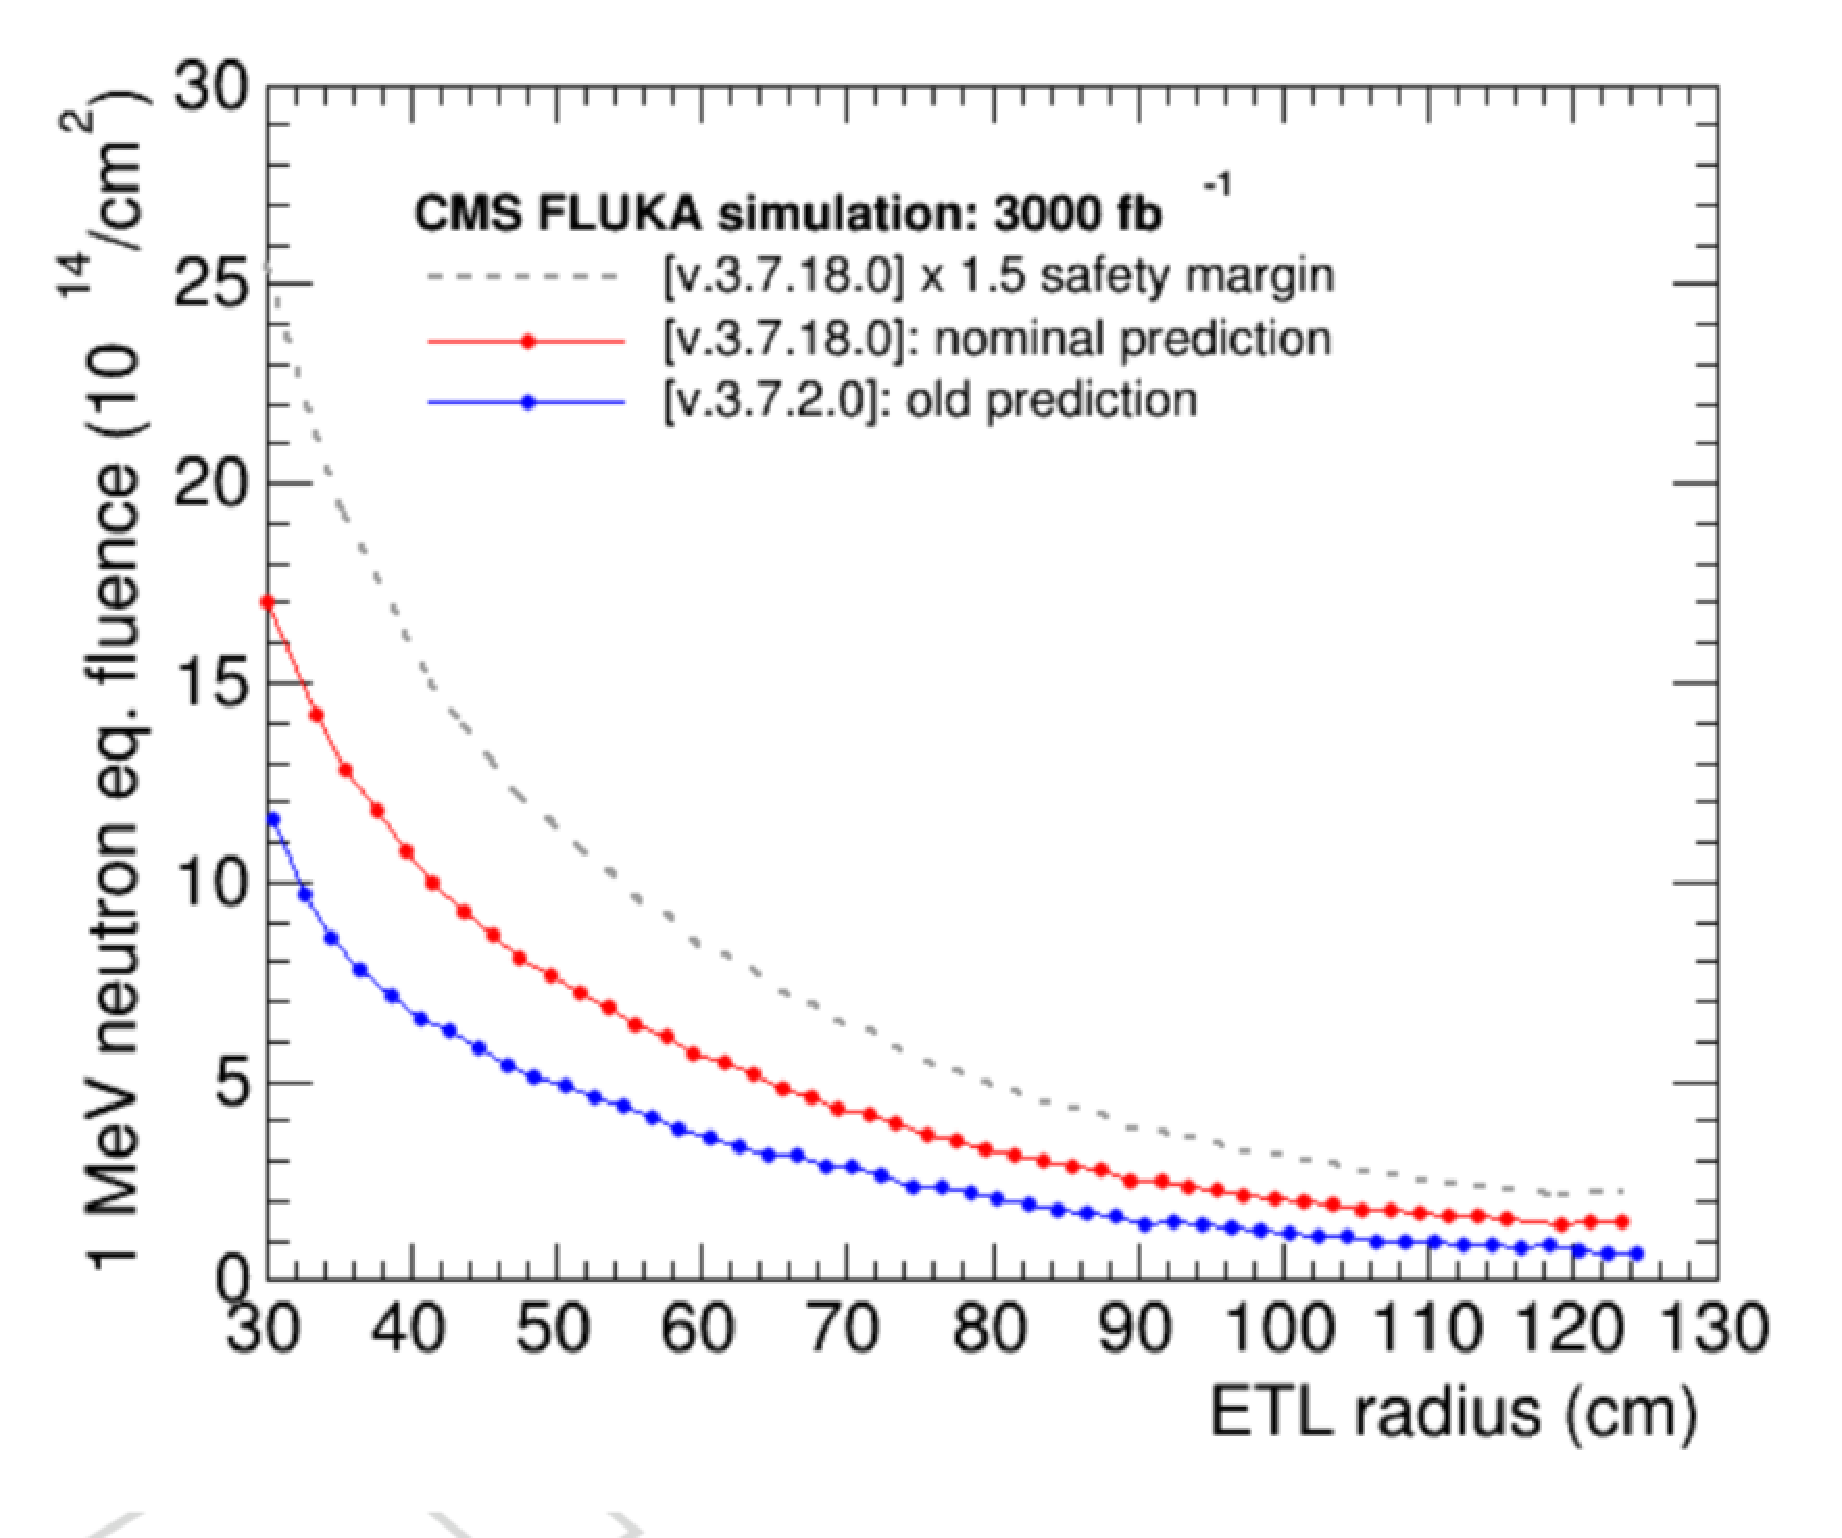
\includegraphics[width=\linewidth]{figures/image6.pdf}

\emph{Figure 6: Fluence prediction in ETL for an integrated luminosity of 3000 fb$^{-1}$ from the FLUKA simulations.}

\section{Geometric Coverage}

Can you reproduce the image below?

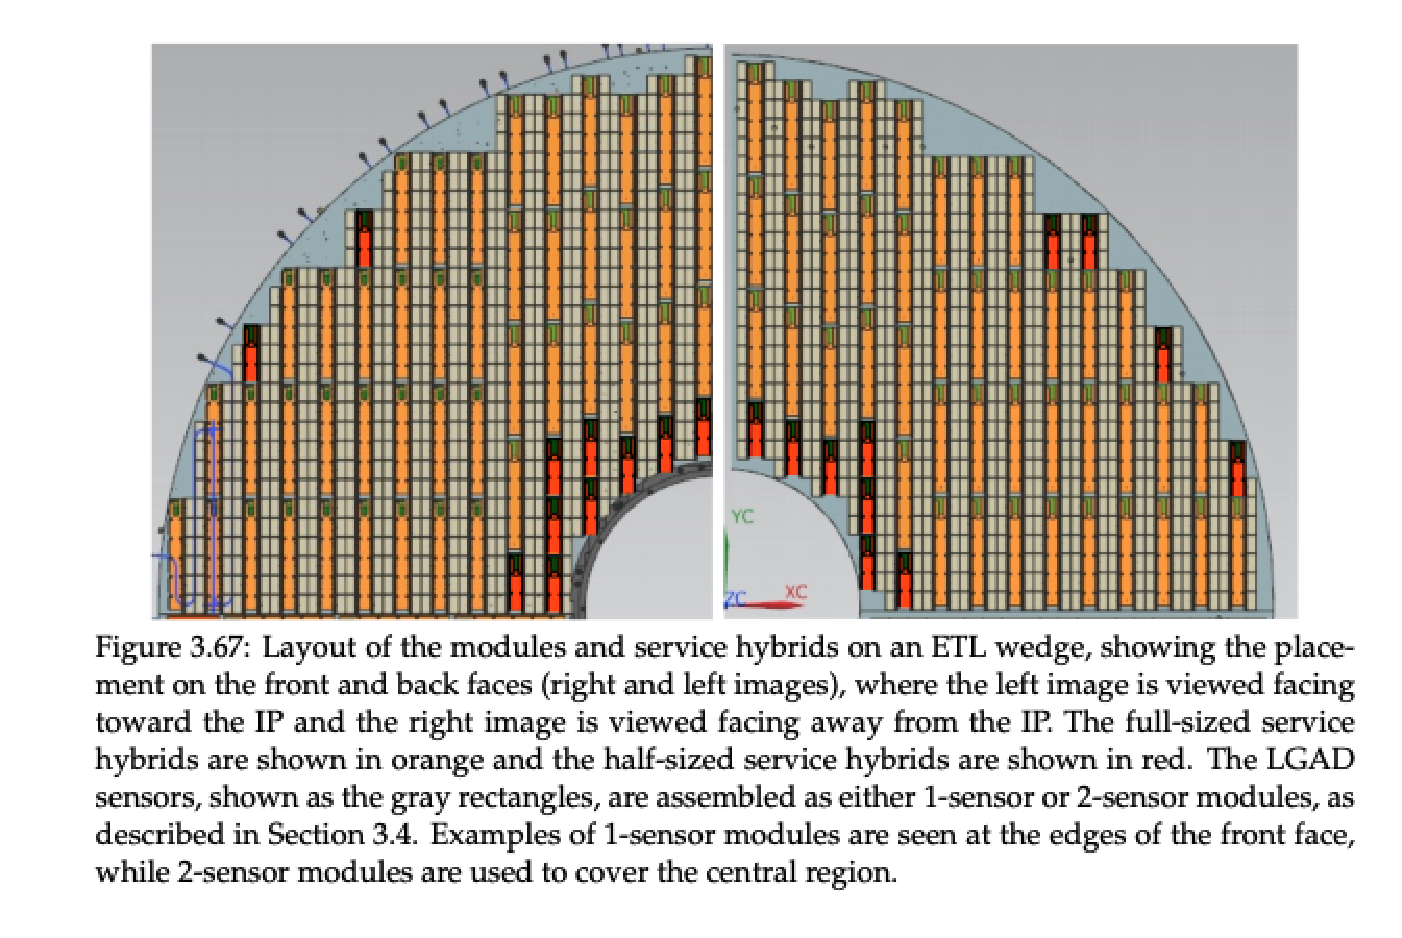
\includegraphics[width=\linewidth]{figures/image5.pdf}

\section{Services}

LV distribution, Bias Voltage, Grounding, Cooling

Can we put Natalia's proposal on the LV PP in here?

\section{Summary}

Summary table comparing the TDR design with the flipped module design. Or a pro/con list

\section{Bibliography}

\begin{itemize}
  \item [1]  C. Collaboration, "A MIP Timing Detector for the CMS Phase-2 Upgrade," CERN-LHCC-2019-003, 2019.
  \item [2]  S. Los, "Proposal for Readout Board on Top ETL SH Stack-up," 23 March 2020. [Online]. Available: https://indico.cern.ch/event/901444.
  \item [3]  A. Apresyan and W. Li, "ETL service hybrid prototyping plan," 2020. [Online]. Available: https://cms-docdb.cern.ch/cgi-bin/DocDB/ShowDocument?docid=14040.
  \item [4]  F. Faccio, "The bPOL12V DCDC converter for HL-LHC trackers: towards production readiness," in \emph{TWEPP}, Santiago de Compostela, 2019.
  \item [5]  J. Troska, A. Brandon-Bravo, S. Detraz, A. Kraxner, L. Olanterä, C. Scarcella, C. Sigaud, C. Soos and F. Vasey, "The VTRx+, an optical link module for data transmission at HL-LHC," in \emph{Topical Workshop on Electronics for Particle Physics}, Santa Cruz,, 2017.
  \item [6]  P. Moreira, "The lpGBT: a radiation tolerant ASIC for Data, Timing, Trigger and Control Applications in HL-LHC," in \emph{TWEPP}, Santiago de Compostela, 2019.
  \item [7]  A. Caratelli, S. Bonacini, K. Kloukinas, A. Marchioro, P. Moreira, R. De Oliveira and C. Paillard, "The GBT-SCA, a radiation tolerant ASIC for detector control and monitoring applications in HEP experiments," \emph{JINST,} vol. 10, no. 03, p. C03034, 2015.
  \item [8]  M. O. Sahin, "DAQ and clock -- status and schedule," in \emph{Timing Days}, CERN, 2020.
  \item [9]  K. DiPetrillo, "ETROC0 Tests with FEAST Based Switching Power Supply," ETL Meeting, 24 Nov 2019. [Online]. Available: https://indico.cern.ch/event/866436/.
  \item [10]  S. Los, "Power board prototyping plans," ETL Meeting, 29 April 2019. [Online]. Available: https://indico.cern.ch/event/816963.
  \item [11]  S. Lusin, "ETL Integration Issues," ETL meeting on sensors and modules, 6 Apr 2020. [Online]. Available: https://indico.cern.ch/event/906805/.
  \item [12]  CERN, "SAFETY INSTRUCTION IS23 - Criteria and Standard Test Methods for the Selection of Electric Cables and Wires with Respect to Fire Safety and Radiation Resistance," CERN, 2005. [Online]. Available:
    https://edms.cern.ch/ui/file/335745/4/E\_IS23.pdf.
  \item [13]  CERN, "Safety Instruction - The use of plastic and other Non-Metallic Materials at CERN with respect to Fire Safety and Radiation Resistance," CERN, 2005. [Online]. Available: https://edms.cern.ch/ui/file/335806/1.02/IS41\_E.pdf.
  \item [14]  P. Moreira, "lpGBT -- a User's Perspective," TWEPP, 17 Sep 2018. [Online]. Available:
  \item [15]  J. Olsen, "ETL DAQ and Fast Control: the view from ETROC/Front-end," ETL meeting (Front-End Electronics), 30 Mar 2020. [Online]. Available: https://indico.cern.ch/event/902740/.
\end{itemize}

\end{document}
